%% Generated by paper_submission/_build/build_tex.js from content_bmc2d.js -- edit the content file,
%% not this file. Springer Nature LaTeX template (sn-jnl, recommended by BMC Medical Imaging), Vancouver
%% numbered references. Submission layout: one column, double spacing, line numbers.
%% BMC compiles submissions with pdfLaTeX (TeX Live 2021). Upload this file, references.bib and figures/.
\documentclass[pdflatex,sn-vancouver-num]{sn-jnl}

\usepackage{graphicx}%
\usepackage{multirow}%
\usepackage{amsmath,amssymb,amsfonts}%
\usepackage{amsthm}%
\usepackage{mathrsfs}%
\usepackage[title]{appendix}%
\usepackage{xcolor}%
\usepackage{textcomp}%
\usepackage{manyfoot}%
\usepackage{booktabs}%
\usepackage{url}%
\raggedbottom
\newcommand{\tbd}[1]{\textcolor{red}{\textbf{[#1]}}}
\usepackage{lineno}
\linenumbers
\usepackage{setspace}
\doublespacing
\setcounter{secnumdepth}{0}

\begin{document}

\title[Single-slice brain tumor segmentation and measurement]{Segmentation, type classification and measurement of brain tumors on single 2D MRI slices: a retrospective development and leakage-controlled internal validation study}

\author*[1]{\fnm{Debobrato} \sur{Biswas}}\email{debobrato095@gmail.com}

\affil*[1]{\orgdiv{Department of Computer Science and Engineering}, \orgname{Daffodil International University}, \orgaddress{\city{Dhaka}, \country{Bangladesh}}}

\abstract{\textbf{Background:} Many brain tumor studies on public two-dimensional (2D) magnetic resonance imaging (MRI) collections report near-perfect classification, yet they rarely localize or measure the tumor, and the two most used collections share images, which can leak test images into training. We developed a model that outlines the tumor on a single 2D slice, names its type and reports its size and side, and evaluated it with patient-level, leakage-controlled splits.

\textbf{Methods:} A U-Net with an ImageNet-pretrained ResNet34 encoder and a four-class head (no tumor, glioma, meningioma, pituitary tumor) was trained on 3064 contrast-enhanced T1-weighted slices with expert masks from 233 patients (figshare dataset) and on class labels from the Kaggle Brain Tumor MRI Dataset. The figshare data were split by patient, and Kaggle images that copy held-out figshare slices were removed. Post-processing derives the longest and perpendicular diameters, the side of the brain and a low-confidence flag. Segmentation was tested on 24 unseen patients (295 slices) and classification on 1311 Kaggle test images, including a subset without copies of training images.

\textbf{Results:} Mean Dice was 0.750 (95\% confidence interval 0.657--0.838; median 0.863): 0.942 for meningioma, 0.801 for pituitary tumor and 0.634 for glioma. The median absolute error of the longest diameter was 3.6 mm, and the side agreed with the expert mask on all 90 axial or coronal slices where the outline overlapped the tumor. Four-class accuracy was 98.9\% (95\% confidence interval 98.4--99.5\%) and tumor detection accuracy 99.77\%, compared with 93.7\% for a 3D detection network applied to the same images. Detection probabilities were well calibrated (expected calibration error 0.023).

\textbf{Conclusions:} A pretrained U-Net delineates and measures meningiomas and pituitary tumors on single slices with errors of a few millimetres, but subtle gliomas at the skull base remain a failure mode. Classification accuracy on the public Kaggle test split is near ceiling and inflated by duplicated images, so localization and measurement are the more informative targets for these datasets.}

\keywords{Brain tumor, Magnetic resonance imaging, Segmentation, U-Net, Transfer learning, Data leakage, Tumor measurement}

\maketitle

\section{Background}\label{sec:background}

Brain and central nervous system tumors caused an estimated 308000 new cases worldwide in 2020~\cite{sung2021globocan}. Their management depends on the tumor type, location and size: the World Health Organization (WHO) classification separates gliomas, meningiomas and pituitary adenomas with very different prognoses~\cite{louis2021who}, and response criteria such as Response Assessment in Neuro-Oncology (RANO) rely on bidimensional diameters measured on contrast-enhanced images~\cite{wen2010rano}. Manual delineation is slow and varies between raters~\cite{menze2015}, which motivates automated support.

Deep learning has been applied widely to brain MRI~\cite{litjens2017}. Two public collections of 2D slices are used particularly often: the figshare dataset of Cheng et al. (3064 contrast-enhanced T1-weighted slices from 233 patients with expert tumor masks)~\cite{cheng2015,cheng2016,cheng2017figshare} and the Kaggle Brain Tumor MRI Dataset, which adds tumor-free images and is organized into training and testing folders~\cite{nickparvar2021kaggle}. Studies on these data mostly address classification and report accuracies close to 100\%~\cite{swati2019,deepak2019}.

Two issues limit what such numbers mean. First, a class label alone does not tell a clinician where the tumor is, how large it is or on which side of the brain; these quantities need a segmentation. Second, the Kaggle collection re-uses figshare slices and contains duplicates across its own training and testing folders, and the figshare slices of one patient are highly correlated. Image-level random splits on such data let near-identical images appear in training and test sets, a well-documented source of optimistic results in medical imaging~\cite{varoquaux2022,roberts2021}.

This study therefore asks how well a single model can (i) outline the tumor on a single 2D slice, (ii) classify it as no tumor, glioma, meningioma or pituitary tumor, and (iii) report its diameters and side, when evaluated on unseen patients with duplicated images removed. The contributions are:

\begin{enumerate}
\item a multi-task U-Net with a pretrained ResNet34 encoder, trained on expert masks and class labels from the two public collections;
\item a leakage-controlled protocol: patient-level splits for the figshare data, removal of Kaggle images that copy held-out figshare slices, and a separate report on the Kaggle test images that do not copy any training image;
\item post-processing that converts the outline into longest and perpendicular diameters, area, side (radiological convention) and a low-confidence flag, with agreement against expert masks;
\item released code, split files and per-image results.
\end{enumerate}

\section{Methods}\label{sec:methods}

\subsection{Study design}

This is a retrospective development and internal-validation study on public, de-identified data. Reporting follows the Checklist for Artificial Intelligence in Medical Imaging (CLAIM)~\cite{mongan2020claim} and the relevant items of TRIPOD+AI~\cite{collins2024tripod}; the completed CLAIM checklist and supplementary tables are given in Additional file 1. Fig. 1 summarizes the system.

\begin{figure}[!t]
\centering
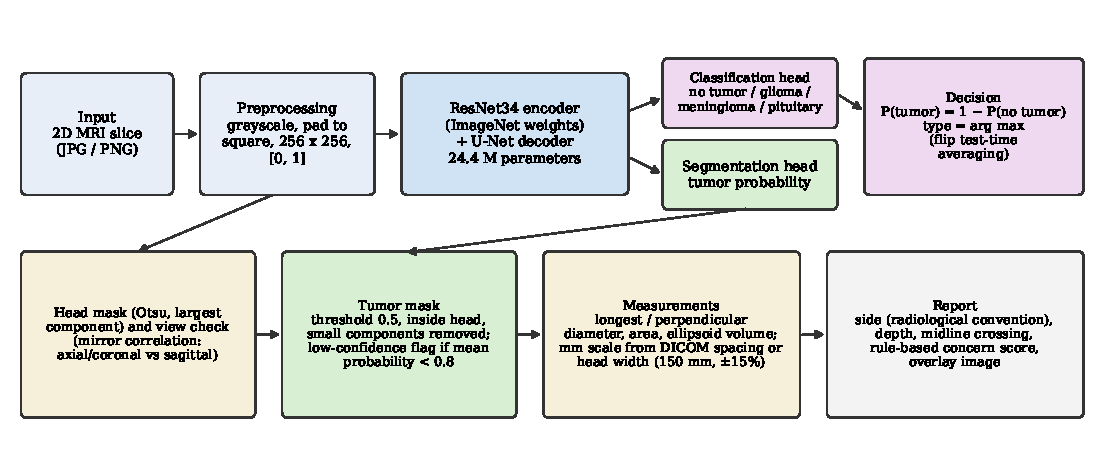
\includegraphics[width=\textwidth]{figures/fig1_pipeline.pdf}
\caption{\textbf{Overview of the segmentation, classification and measurement system.} A 2D slice is converted to a 256 $\times$ 256 grayscale input. A U-Net with a pretrained ResNet34 encoder predicts a tumor probability map and four class probabilities. Post-processing restricts the mask to the head, removes small components, flags low-confidence outlines and derives diameters, area, side and depth. Without pixel spacing, the millimetre scale is estimated from the head width.}\label{fig1}
\end{figure}

\subsection{Datasets}

\textbf{figshare brain tumor dataset}~\cite{cheng2015,cheng2016,cheng2017figshare}: 3064 contrast-enhanced T1-weighted slices (axial, coronal and sagittal) from 233 patients with meningioma (708 slices), glioma (1426) or pituitary tumor (930), each with a tumor mask drawn by experts. The dataset documentation states a pixel size of 0.49 mm at 512 $\times$ 512 pixels.

\textbf{Kaggle Brain Tumor MRI Dataset}~\cite{nickparvar2021kaggle}: 2D images in four classes (glioma, meningioma, pituitary, no tumor) with a Training folder (5712 images) and a Testing folder (1311 images: 906 with tumor and 405 without). It has no masks and no patient identifiers, and part of its tumor images are taken from figshare.

\subsection{Data splits and leakage control}

The figshare patients were split at random (seed 42) into training (186 patients, 2439 slices), validation (23 patients, 330 slices) and test (24 patients, 295 slices) sets, so no patient contributes to more than one set; the split is listed in Additional file 2. Images were compared after resizing to 32 $\times$ 32 pixels and per-image z-scoring; a mean absolute difference below 0.08 was treated as a copy (copies measured below 0.05 and different slices above 0.1). 305 Kaggle Training images that copy a figshare validation or test slice were removed; of the rest, 4867 were used for training and 540 for validation. In the Kaggle Testing folder, 621 images copy a figshare training slice or a Kaggle Training image; results are reported for all 1311 images and for the 690 images without a copy (Additional file 1: Table S2).

\subsection{Preprocessing}

Each image was converted to grayscale, zero-padded to a square around its center (so one pixel covers the same distance horizontally and vertically), resized to 256 $\times$ 256 pixels and scaled to [0, 1]. The figshare slices were first min--max scaled to 8 bits, as in the public JPEG versions.

\subsection{Model}

The network is a U-Net~\cite{ronneberger2015} whose encoder is a ResNet34~\cite{he2016resnet} initialized with ImageNet weights~\cite{deng2009imagenet} (the grayscale input is repeated over three channels and normalized with ImageNet statistics). Four decoder stages upsample bilinearly, concatenate the encoder features of matching resolution and apply two 3 $\times$ 3 convolutions with batch normalization and rectified linear units; the segmentation head (3 $\times$ 3 convolution with batch normalization, rectified linear unit and a 1 $\times$ 1 convolution) outputs one logit per pixel at full resolution. A classification head (dropout 0.3, linear layer) on the globally pooled deepest encoder features outputs four logits. The model has 24.4 million parameters.

\subsection{Training}

Each epoch used all 2439 figshare training slices and 1500 Kaggle training images drawn at random. The figshare slices contribute both losses; Kaggle tumor images contribute only the classification loss, and Kaggle no-tumor images contribute both with an empty mask. The loss is binary cross-entropy plus soft Dice~\cite{milletari2016vnet} (Dice only on images with tumor) plus 0.5 $\times$ weighted cross-entropy with label smoothing 0.05. Optimization used AdamW~\cite{loshchilov2019adamw} (weight decay 10\textsuperscript{$-$4}), a one-cycle learning-rate schedule with maximum 3 $\times$ 10\textsuperscript{$-$4}~\cite{smith2019onecycle}, batch size 12 and up to 12 epochs. Augmentation comprised horizontal flips, rotation ($\pm$15$^\circ$), scaling (0.85--1.15), translation ($\pm$8\%), gamma (0.7--1.5), contrast and brightness changes, Gaussian blur and noise. The checkpoint with the highest sum of validation Dice (figshare) and validation accuracy (Kaggle) was kept (epoch 11; validation Dice 0.792). Training ran on a 12-core central processing unit in PyTorch~\cite{paszke2019pytorch}, about 13 min per epoch; all hyper-parameters and software versions are listed in Additional file 1: Table S3.

\subsection{Inference and post-processing}

At inference the prediction is averaged with that of the horizontally flipped image. The tumor probability is P(tumor) = 1 $-$ P(no tumor) from the classification head, and the type is the most probable class. The head is segmented by Otsu thresholding~\cite{otsu1979} of the smoothed image (largest component, holes filled). The tumor mask is the probability map thresholded at 0.5, restricted to the head, without components smaller than 25 pixels or 10\% of the largest component. The longest diameter is the largest distance between mask pixels (Feret diameter); the perpendicular diameter is the extent orthogonal to it. Area follows from the pixel count, and a volume estimate assumes an ellipsoid whose third axis equals the perpendicular diameter~\cite{kothari1996}.

Side is reported in the radiological convention (image left = patient right) from the horizontal offset of the tumor centroid relative to the head midline; offsets within 8\% of the half-width are reported as midline. Because left and right are undefined on sagittal slices, the view is checked by the correlation between the head region and its mirror image: below 0.5 the slice is treated as sagittal and no side is given; between 0.5 and 0.7 the side is reported as conditional. JPEG and PNG files carry no pixel spacing; when none is supplied, the millimetre scale is estimated by assuming a head width of 150 mm on axial and coronal slices, close to the adult head breadth in anthropometric surveys~\cite{gordon2014ansur}. An outline whose mean probability is below 0.8 is flagged as uncertain. A rule-based concern score (size, type, depth, midline involvement, ring pattern) is shown in the software but was not evaluated and is not part of the results.

\subsection{Evaluation and statistics}

Segmentation was evaluated on the figshare test patients against the expert masks with the Dice coefficient~\cite{dice1945}, intersection over union (IoU), precision, recall and the 95th-percentile Hausdorff distance (HD95), following current recommendations for segmentation metrics~\cite{maierhein2024metrics} and using the nominal pixel size of the 256-pixel images (0.98 mm). Diameters were computed identically on predicted and expert masks and compared with Bland--Altman analysis~\cite{bland1986}. Side agreement was assessed on axial or coronal test slices whose expert-mask centroid lies outside the midline band. Confidence intervals (CI) for segmentation metrics come from 2000 bootstrap resamples of patients~\cite{efron1993bootstrap}, because slices of one patient are not independent; those for classification come from 2000 image-level resamples. Classification and detection were evaluated on the Kaggle Testing folder (accuracy, sensitivity, specificity, area under the receiver operating characteristic curve (AUC), per-class F1) and compared with a 3D convolutional detection network (squeeze-and-excitation 3D U-Net encoder) trained earlier in the same project on the same Kaggle training images. Calibration of P(tumor) was measured with the expected calibration error (ECE) over ten bins~\cite{guo2017calibration}. Ablations varied the mask threshold (0.3, 0.5, 0.7) and test-time flipping.

\section{Results}\label{sec:results}

\subsection{Segmentation}

On 295 slices from 24 unseen patients, the mean Dice was 0.750 (95\% CI 0.657--0.838) and the median 0.863 (Table 1). Of the slices, 85.8\% reached Dice $\geq$ 0.5; on 26 slices the outline missed the tumor (Dice < 0.1), and on 3 no outline was produced. Performance differed by tumor type: meningiomas were delineated best (Dice 0.942), pituitary tumors well (0.801), and gliomas least well (0.634; Table 2). Fig. 2 shows the best, median and worst slice of each type, and the result for every test slice is listed in Additional file 3.

\begin{table}[!t]
\caption{Segmentation performance on the figshare test patients}\label{tab1}
\centering\footnotesize
\begin{tabular}{lc}
\toprule
Metric & Proposed (pretrained ResNet34 U-Net) \\
\midrule
Dice & 0.750 [0.657--0.838] (0.863) \\
IoU & 0.663 [0.573--0.764] (0.759) \\
Precision & 0.774 [0.682--0.862] \\
Recall & 0.772 [0.682--0.856] \\
HD95 (mm) & 15.2 [8.4--23.0] (5.8) \\
Slices with Dice $\geq$ 0.5 (\%) & 85.8 \\
Parameters (millions) & 24.4 \\
\botrule
\end{tabular}
\footnotetext{24 patients, 295 slices. Values are means with patient-level bootstrap 95\% CI in brackets and medians in parentheses. Post-processing: threshold 0.5, mask restricted to the head. IoU, intersection over union; HD95, 95th-percentile Hausdorff distance (nominal 0.98 mm pixels).}
\end{table}

\begin{table}[!t]
\caption{Segmentation performance by tumor type on the figshare test patients}\label{tab2}
\centering\footnotesize
\begin{tabular}{lccc}
\toprule
Type & Patients / slices & Dice mean [95\% CI] & Median Dice / HD95 (mm) \\
\midrule
Meningioma & 10 / 88 & 0.942 [0.923--0.953] & 0.953 / 1.4 \\
Pituitary tumor & 3 / 43 & 0.801 [0.718--0.859] & 0.851 / 2.9 \\
Glioma & 11 / 164 & 0.634 [0.498--0.723] & 0.755 / 14.5 \\
\botrule
\end{tabular}
\footnotetext{CI, patient-level bootstrap confidence interval; HD95, 95th-percentile Hausdorff distance.}
\end{table}

\begin{figure}[!t]
\centering
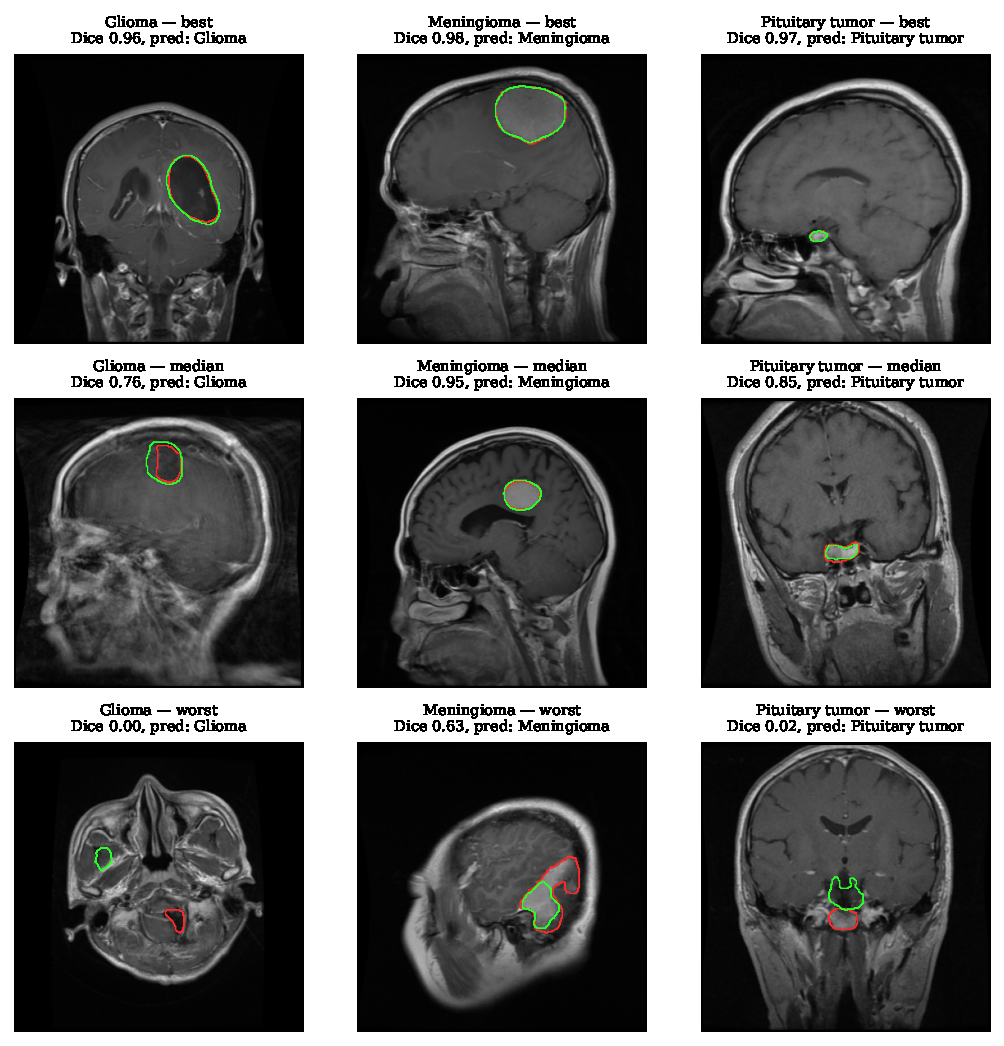
\includegraphics[width=\textwidth]{figures/fig3_qualitative.pdf}
\caption{\textbf{Best, median and worst test slice of each tumor type.} Rows show the best (top), median (middle) and worst (bottom) test slice of each tumor type ranked by Dice. Red, expert mask; green, model outline. The worst glioma lies in the posterior fossa and the model outlines the temporal lobe instead; in the worst pituitary case the model outlines tissue above the tumor.}\label{fig2}
\end{figure}

\subsection{Size and side}

On the 292 test slices with an outline, the median absolute error of the longest diameter was 3.6 mm (median relative error 8.2\%), the mean absolute error 9.4 mm, the bias -0.8 mm and the correlation r = 0.72 (Fig. 3). Restricted to the 269 outlines that overlap the tumor, the bias was -0.1 mm with limits of agreement from -30.1 to 29.9 mm: most errors are small, but a minority of large errors, mainly irregular gliomas outlined too widely or too narrowly, widens the limits. Tumor area correlated with r = 0.79 (median relative error 14.6\%).

The side agreed with the expert mask on 90.4\% of 104 eligible slices; all disagreements came from outlines that missed the tumor, and agreement was 100\% on the 90 slices where the outline overlapped it. With the scale estimated from the head width, the estimated pixel size was 0.84 times the nominal 0.98 mm in the median (10th--90th percentile 0.73--0.98; Additional file 1: Table S5); the nominal spacing implies a median head width of about 180 mm, larger than typical adult head breadth, so either the nominal spacing does not hold for all slices or the 150 mm assumption is too small. Sizes from images without pixel spacing should therefore be read as approximate.

\begin{figure}[!t]
\centering
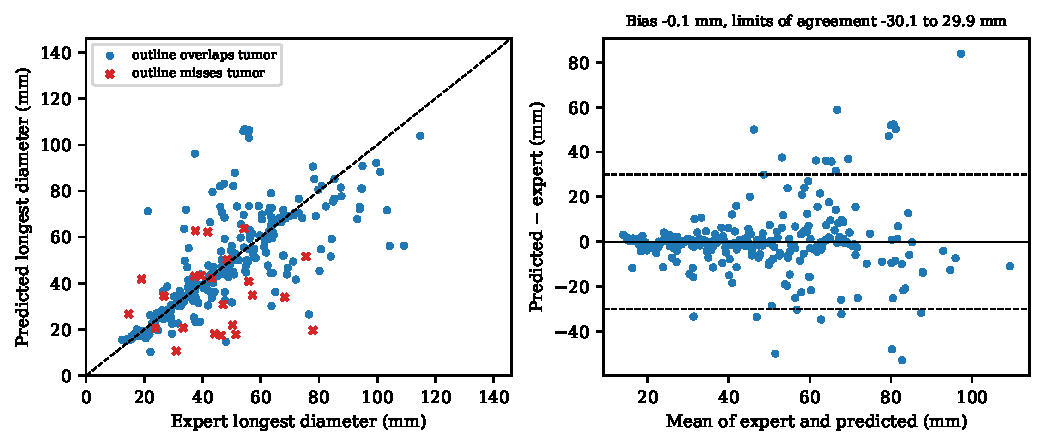
\includegraphics[width=\textwidth]{figures/fig4_diameter_agreement.pdf}
\caption{\textbf{Agreement of the longest tumor diameter between model and expert masks.} Figshare test patients, nominal pixel size. Left: scatter plot of predicted versus expert longest diameter; crosses mark outlines that miss the tumor. Right: Bland--Altman plot for outlines that overlap the tumor; the solid line is the mean difference and the dashed lines are the 95\% limits of agreement.}\label{fig3}
\end{figure}

\subsection{Classification and detection}

On all 1311 Kaggle test images the four-class accuracy was 98.9\% (95\% CI 98.4--99.5\%) with macro-F1 0.989 (Fig. 4; per-class results in Additional file 1: Table S4); on the 690 images without a copy in training it was 98.8\%. For tumor versus no tumor, the model reached 99.77\% accuracy, 99.89\% sensitivity and 99.51\% specificity (Table 3), with 1 missed tumor and 2 false positives. The 3D detection network missed 70 tumors (sensitivity 92.3\%), and averaging both models was worse than the 2D model alone. The type was correct on 99.3\% of figshare test slices. The prediction for every Kaggle test image is listed in Additional file 4.

\begin{table}[!t]
\caption{Tumor detection on the Kaggle Testing folder}\label{tab3}
\centering\footnotesize
\begin{tabular}{lccccc}
\toprule
Model & Accuracy (\%) & Sens. (\%) & Spec. (\%) & AUC & ECE \\
\midrule
Proposed (2D) & 99.77 [99.47--100.00] & 99.89 & 99.51 & 0.9999 & 0.023 \\
3D detection network & 93.67 [92.37--94.97] & 92.27 & 96.79 & 0.9850 & 0.026 \\
Mean of both & 98.55 & 98.90 & 97.78 & 0.9991 & --- \\
Proposed, no copies (n = 690) & 100.00 & 100.00 & 100.00 & 1.0000 & --- \\
3D network, no copies (n = 690) & 98.12 & 98.04 & 100.00 & 0.9943 & --- \\
\botrule
\end{tabular}
\footnotetext{906 images with tumor and 405 without; image-level bootstrap 95\% CI in brackets. "No copies" excludes test images that copy a training image; it contains only 28 tumor-free images, so its specificity is imprecise. Sens., sensitivity; Spec., specificity; AUC, area under the receiver operating characteristic curve; ECE, expected calibration error.}
\end{table}

\begin{figure}[!t]
\centering
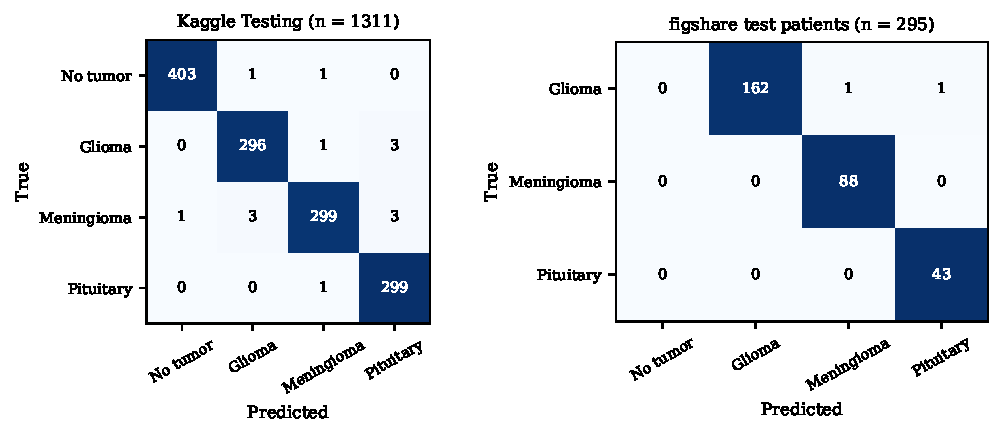
\includegraphics[width=\textwidth]{figures/fig5_confusion.pdf}
\caption{\textbf{Confusion matrices of the classification head.} Left: Kaggle Testing folder, four classes. Right: tumor type on the figshare test patients, which contain no tumor-free slices. Numbers are image counts; shading is the row-normalized proportion.}\label{fig4}
\end{figure}

\subsection{Calibration, ablations, flag and run time}

The expected calibration error of P(tumor) was 0.023 (Fig. 5). Without test-time flipping the mean Dice was 0.755 at threshold 0.5 (0.756 at 0.3, 0.753 at 0.7), and with flipping 0.750 (0.755 and 0.743; Additional file 1: Table S6): flipping did not improve segmentation and the result is insensitive to the threshold. Of 618 outlines on validation and test slices, 39 missed the tumor; the low-confidence flag marked 15 of them and 11 correct outlines (the threshold was chosen on these slices, so this is descriptive). A full analysis of one image took 0.15 s (median) on 6 processor threads. Fig. 6 shows the output for two test patients.

\begin{figure}[!t]
\centering
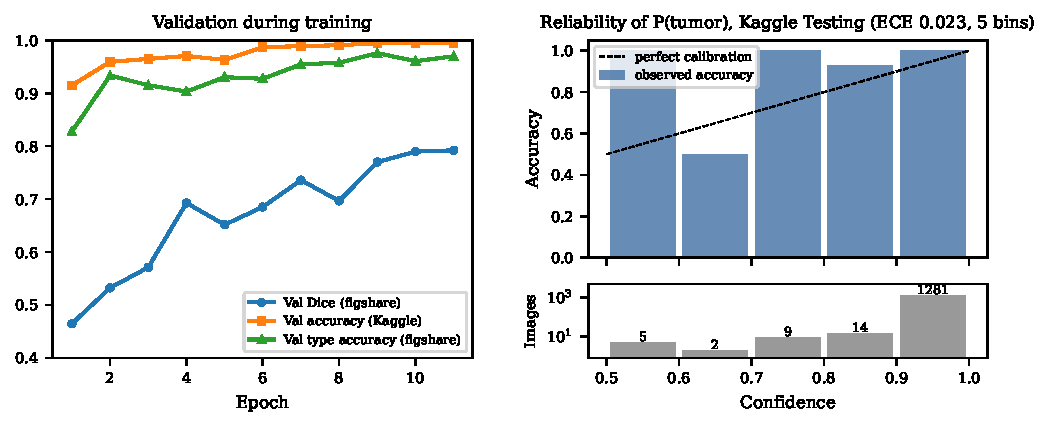
\includegraphics[width=\textwidth]{figures/fig6_training_calibration.pdf}
\caption{\textbf{Validation metrics during training and calibration of the tumor probability.} Left: validation Dice (figshare) and validation accuracies during training. Right: reliability diagram of P(tumor) on the Kaggle Testing folder with five confidence bins; the lower panel gives the number of images per bin on a log scale. The low-confidence bins hold few images, so their accuracies are imprecise.}\label{fig5}
\end{figure}

\begin{figure}[!t]
\centering
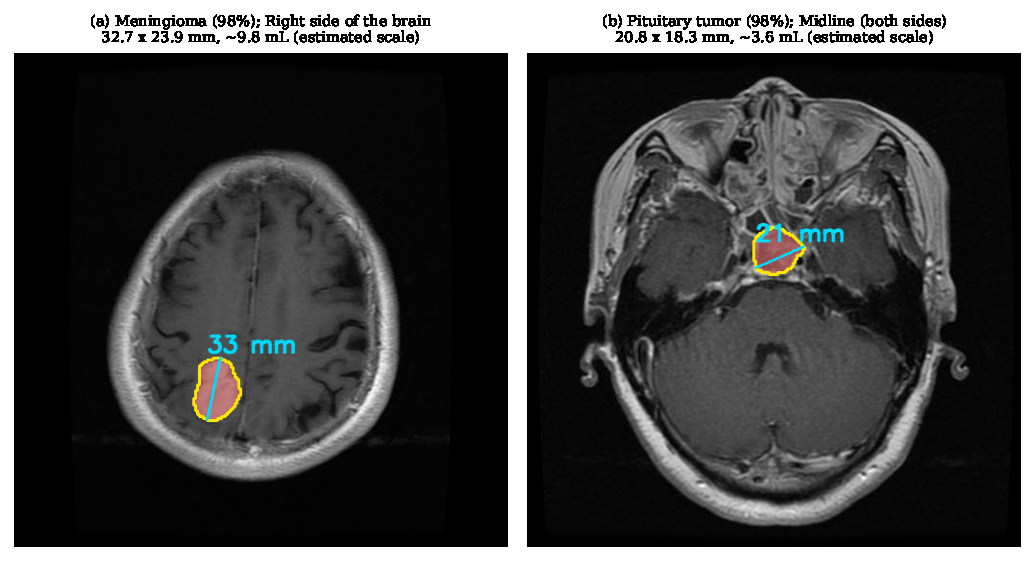
\includegraphics[width=\textwidth]{figures/fig7_example_output.pdf}
\caption{\textbf{System output for two unseen test patients.} Each panel shows the outline, the longest diameter, the side, the predicted type and the estimated size, with the scale estimated from the head width. Expert longest diameters measured on the corresponding figshare masks at the same estimated scale are 32.2 mm (a) and 19.9 mm (b).}\label{fig6}
\end{figure}

\section{Discussion}\label{sec:discussion}

A U-Net with a pretrained ResNet34 encoder, trained on fewer than 2500 slices with masks, delineated meningiomas (Dice 0.94) and pituitary tumors (0.80) on unseen patients and measured the longest tumor diameter with a median error of 3.6 mm. The side of the brain was always right when the outline overlapped the tumor, so side errors reduce to segmentation failures, which the low-confidence flag catches only in part.

Gliomas were the hardest type. They are infiltrative and often heterogeneous, and several failures in this test set lie at the skull base or in the posterior fossa, where vessels, sinuses and bone also enhance on contrast-enhanced T1-weighted images. The worst cases in Fig. 2 show the typical failure: an enhancing structure elsewhere is outlined instead of the tumor. Expert masks of gliomas also sometimes include the non-enhancing surrounding tissue, whereas the model tends to outline the enhancing part only, which lowers both Dice and the measured diameter.

Classification results illustrate why localization is the more informative target. Four-class accuracy (98.9\%) and detection accuracy (99.77\%) are near ceiling, as in prior reports on these data~\cite{swati2019,deepak2019}. However, 621 of the 1311 Kaggle test images copy a training image, and the remaining subset holds only 28 tumor-free images. Patient identifiers are missing from the Kaggle data, so near-duplicates from the same patient cannot be excluded completely. Accuracy on this split mainly shows that the model recognizes images from the same sources and should not be read as a measure of clinical performance~\cite{varoquaux2022,roberts2021}. The segmentation results, by contrast, come from patients never seen in training.

Measurements from 2D images have two further limits. Without pixel spacing from the Digital Imaging and Communications in Medicine (DICOM) header the scale must be estimated; the head-width assumption introduces an error of the order of 15\%, and the documented spacing of the source data itself appears inconsistent with typical head sizes. A single slice also gives no third dimension, so volumes are ellipsoid approximations and the measured diameter depends on which slice was chosen. Clinical response assessment requires the slice with the largest tumor extent and consistent acquisition~\cite{wen2010rano}.

\subsection{Limitations}

\begin{enumerate}
\item Internal validation only: both datasets are public, partly overlapping and acquired at few centers; no external test set was used.
\item One contrast (contrast-enhanced T1-weighted) and three tumor types; other tumors, other sequences, post-operative scans, photographs of film and screenshots are out of scope.
\item The figshare test set has 24 patients and the pituitary group only 3, so its confidence interval is wide.
\item Single training run and seed; no hyper-parameter search; no segmentation baseline (for example a classic U-Net or the self-configuring nnU-Net~\cite{isensee2021nnunet}) was trained on the same split, so the segmentation accuracy is not compared with other methods under identical conditions.
\item Size estimates without pixel spacing are approximate, and the concern score shown by the software is rule-based and not validated.
\end{enumerate}

\section{Conclusions}\label{sec:conclusions}

On single 2D contrast-enhanced T1-weighted slices, a pretrained U-Net outlines meningiomas and pituitary tumors close to expert masks and reports their diameter and side with small errors, while subtle gliomas at the skull base remain a failure mode. With leakage controlled, near-perfect classification on the public Kaggle split adds little information; localization and measurement on patient-level splits are the more meaningful benchmarks. External validation on DICOM data with known pixel spacing is the next step before any clinical use.

\backmatter

\bmhead{Abbreviations}
2D/3D, two-/three-dimensional; AUC, area under the receiver operating characteristic curve; CI, confidence interval; CLAIM, Checklist for Artificial Intelligence in Medical Imaging; DICOM, Digital Imaging and Communications in Medicine; ECE, expected calibration error; HD95, 95th-percentile Hausdorff distance; IoU, intersection over union; MRI, magnetic resonance imaging; RANO, Response Assessment in Neuro-Oncology; WHO, World Health Organization.

\section*{Declarations}
\bmhead{Ethics approval and consent to participate}
Not applicable. The study used only publicly available, de-identified datasets (figshare brain tumor dataset; Kaggle Brain Tumor MRI Dataset) released by their creators for research; no new data were collected from humans.

\bmhead{Consent for publication}
Not applicable.

\bmhead{Availability of data and materials}
The datasets supporting the conclusions of this article are available in the figshare repository, \url{https://doi.org/10.6084/m9.figshare.1512427}~\cite{cheng2017figshare}, and in the Kaggle repository, \url{https://doi.org/10.34740/KAGGLE/DSV/2645886}~\cite{nickparvar2021kaggle}. The patient-level split, the per-slice segmentation results and the per-image classification results supporting the conclusions of this article are included within its additional files (Additional files 2--4). Software: project name, BrainTumorDetection; project home page, \url{https://github.com/Debobrato06/BrainTumorDetection}~\cite{biswas2026repo}; archived version, \tbd{TBD: Zenodo DOI of the release}; operating system, platform independent (tested on Windows 11); programming language, Python 3.12; other requirements, PyTorch 2.5.1, torchvision 0.20.1, NumPy 2.3.5, SciPy 1.17.0, scikit-image 0.26.0, OpenCV 4.13; license, \tbd{TBD: e.g. MIT}; restrictions to use by non-academics, none. The trained model weights are available from the corresponding author on request.

\bmhead{Competing interests}
The author declares no competing interests.

\bmhead{Funding}
No funding was received for this study or for the publication fees.

\bmhead{Authors' contributions}
DB conceived and designed the study, implemented the software, performed the experiments and analysis, and wrote and revised the manuscript. The author read and approved the final manuscript.

\bmhead{Acknowledgements}
The author thanks Jun Cheng and colleagues and Msoud Nickparvar for making their datasets publicly available.

\bibliography{references}

\section*{Additional files}
\bmhead{Additional file 1 (.pdf)}
\emph{Supplementary tables and CLAIM checklist.} Table S1, completed CLAIM checklist with the location of each item; Table S2, dataset partitions and leakage control; Table S3, training hyper-parameters and software versions; Table S4, per-class classification metrics; Table S5, measurement, side and scale-estimation details; Table S6, threshold and test-time flipping ablation.

\bmhead{Additional file 2 (.csv)}
\emph{Patient-level split of the figshare dataset.} One row per figshare patient identifier with its partition (training, validation or test) and number of slices.

\bmhead{Additional file 3 (.csv)}
\emph{Segmentation and measurement results for every figshare test slice.} For each test slice: file name, patient identifier, true and predicted type, Dice, intersection over union, precision, recall, 95th-percentile Hausdorff distance, expert and predicted diameters and areas, and side offsets.

\bmhead{Additional file 4 (.csv)}
\emph{Classification results for every Kaggle test image.} For each Kaggle Testing image: file path, true and predicted class, tumor probability of the proposed model and of the 3D detection network, copy-of-training-image flag and the four class probabilities.

\end{document}
